\pdfobjcompresslevel 0
\documentclass[10pt, a4paper, parskip=full, twoside, twocolumn]{report}

% --- PREAMBULE ---
\usepackage[utf8]{inputenc}
\usepackage[T1]{fontenc}
\usepackage[french]{babel}
\usepackage{amsmath, amssymb, amsthm, amsfonts}
\usepackage[top=1cm,bottom=2cm,left=1cm,right=1cm]{geometry}
\usepackage{graphicx}
\usepackage{stmaryrd}
\usepackage{xcolor}
\usepackage{framed}
\usepackage{enumitem}
\usepackage{titlesec}
\usepackage{aliascnt}
\usepackage{tcolorbox} % The main package for creating the colored box
\tcbuselibrary{breakable}

% Define a custom color (optional, but good practice)
\definecolor{mygreen}{rgb}{0.2, 0.7, 0.2}
\definecolor{myblue}{rgb}{0.0, 0.2, 0.7}
\definecolor{myred}{rgb}{0.7, 0.2, 0.2}
\definecolor{developpement}{RGB}{255, 255, 224}

% Apply the color to the subsection title
\titleformat{\section}
  {\normalfont\large\bfseries\color{myred}} % The format for the whole line
  {\thesection}                           % The subsection number
  {1em}                                      % Separation between number and title
  {}                                         % Code before the title text (empty for now)

% Apply the color to the subsection title
\titleformat{\subsection}
  {\normalfont\large\bfseries\color{mygreen}} % The format for the whole line
  {\thesubsection}                           % The subsection number
  {1em}                                      % Separation between number and title
  {}                                         % Code before the title text (empty for now)
  
\newtheorem{definition}{Définition}
\newtheorem{theorem}[definition]{Théorème}
\newtheorem{theorem_def}[definition]{Théorème et définition}
\newtheorem{proposition}[definition]{Proposition}
\newtheorem{properties}[definition]{Propriétés}
\newtheorem{property}[definition]{Propriété}
\newtheorem{lemme}[definition]{Lemme}
\newtheorem{corollary}[definition]{Corollaire}
\newtheorem{example}[definition]{Exemple}
\newtheorem{remark}[definition]{Remarque}
\newtheorem{application}[definition]{Application}
\newtheorem{reference}[definition]{Référence}
\newtheorem{algorithm}[definition]{Algorithme}
\newtheorem{notation}[definition]{Notation}
\newtheorem*{notation*}{Notation}

\newcommand{\IN}{\mathbb{N}}
\newcommand{\IZ}{\mathbb{Z}}
\newcommand{\IU}{\mathbb{U}}
\newcommand{\IK}{\mathbb{K}}
\newcommand{\IZnZ}{\mathbb{Z}/n\mathbb{Z}}
\newcommand{\IZpZ}{\mathbb{Z}/p\mathbb{Z}}
\newcommand{\IQ}{\mathbb{Q}}
\newcommand{\IC}{\mathbb{C}}
\newcommand{\IR}{\mathbb{R}}
\newcommand{\IRn}{\mathbb{R}^n}
\newcommand{\IRd}{\mathbb{R}^d}
\newcommand{\IRm}{\mathbb{R}^m}
\newcommand{\IRp}{\mathbb{R}^p}
\newcommand{\IRnm}{\mathbb{R}^{n\times m}}
\newcommand{\IRmn}{\mathbb{R}^{m\times n}}
\newcommand{\IRpn}{\mathbb{R}^{p\times n}}
\newcommand{\IRnp}{\mathbb{R}^{n\times p}}
\newcommand{\IRpm}{\mathbb{R}^{p\times m}}
\newcommand{\IRmp}{\mathbb{R}^{m\times p}}
\newcommand{\actson}{\circlearrowleft}

\DeclareMathOperator{\im}{Im}
% \DeclareMathOperator{\Im}{Im}
\DeclareMathOperator{\pgcd}{pgcd}
\DeclareMathOperator{\ppcm}{ppcm}
\DeclareMathOperator{\card}{Card}
\DeclareMathOperator{\Is}{Is}
\DeclareMathOperator{\Orb}{Orb}
\DeclareMathOperator{\Stab}{Stab}
\DeclareMathOperator{\Fix}{Fix}
\DeclareMathOperator{\Supp}{Supp}
\DeclareMathOperator{\ord}{ord}
\DeclareMathOperator{\Ker}{Ker}
\DeclareMathOperator{\Syl}{Syl}

\titleformat{\chapter}[display]
  {\normalfont\bfseries}{}{0pt}{\LARGE}
\titlespacing*{\chapter}{0pt}{0pt}{\baselineskip}



\title{Leçons d'oral de l'Agrégation}
\author{Gautier Laisné}
\date{}


\begin{document}
% \maketitle
% \tableofcontents

\chapter{101 : Groupe opérant sur un ensemble. Exemples d'applications.}
Dans cette leçon, $G$ désigne un groupe de neutre $1$, et $X$ désigne un ensemble.
\section*{I. Action d'un groupe sur un ensemble}
\subsection*{A. Définitions et premiers exemples}
\begin{definition}[\textnormal{[R] 19, [U] 27}]
	Une \emph{action} de $G$ sur $X$ est une application $G\times X\to X$ définie par 
	$(g,x)\mapsto g\cdot x$ vérifiant
	\begin{enumerate}
		\item $\forall\, (g,g')\in G^2,\, \forall\, x\in X,\, g'\cdot (g\cdot x) = (g'g)\cdot x$
		\item $\forall\, x\in X,\, 1\cdot x = x$
	\end{enumerate}
	Pour signigier que $G$ agit sur $X$, on note $G\actson X$.
\end{definition}

\begin{example}[\textnormal{[R] 19, [U] 28}]
	\begin{itemize}
		\item $\mathfrak{S}(X) \actson X$ par $\sigma\cdot x = \sigma(x)$
		\item Si $E$ est un espace vectoriel, alors $GL(E)\actson E$ par $\varphi\cdot x = \varphi(x)$
		\item $(g,x)\mapsto x$ est une action de $G$ sur $X$, appelée \emph{action triviale}.
	\end{itemize}
\end{example}

\begin{proposition}[\textnormal{[R] 19, [U] 28}]
	La donnée d'une action $(g,x)\mapsto g\cdot x$ de $G$ sur $X$ équivaut à la donnée d'un morphisme $\varphi\,\colon G\to \mathfrak{S}(X)$, $g\mapsto \left[x\mapsto g\cdot x\right]$, appelé \emph{morphisme associé à l'action de $G$ sur $X$}.
\end{proposition}

\begin{definition}[\textnormal{[R] 19/21, [U] 29}]
	Soit $x\in X$. Alors :
	\begin{itemize}
		\item L'\emph{orbite} de $x$ est l'ensemble $\Orb(x) = \left\{g\cdot x \mid g\in G\right\}$ (aussi noté $G\cdot x$) ;
		\item Le \emph{stabilisateur} de $x$ est l'ensemble $\Stab(x) = \left\{g\in G \mid g\cdot x = x\right\}$.
	\end{itemize}
\end{definition}

\begin{proposition}[\textnormal{[U] 34/37}]
	\begin{enumerate}
		\item $G\actson G$ par $g\cdot h=ghg^{-1}$ (on l'appelle \emph{action par conjugaison}). Le stabilisateur de $h\in G$ est appelé \emph{centralisateur} de $h$, et est noté $C(h)$.
		\item $G$ agit sur l'ensemble de ses sous-groupes par $g\cdot H = gHg^{-1}$ (action par conjugaison). Le stabilisateur de $H\leq G$ est appelé \emph{normalisateur} de $H$, et est noté $N(H)$.
	\end{enumerate}
\end{proposition}

\begin{definition}[\textnormal{[R] 20, [U] 29/31}]
	On dit que l'action de $G$ sur $X$ est \emph{transitive} si elle n'a qu'une seule orbite, \emph{i.e.} si $\forall\,(x,y)\in X^2,\, \exists\, g\in G\,\colon g=g\cdot x$.

	On dit que l'action de $G$ sur $X$ est \emph{fidèle} si $\varphi$ est injective.
\end{definition}

\begin{example}[\textnormal{[U] 31}]
	\begin{itemize}
		\item $\mathfrak{S}_n\actson \llbracket 1,n\rrbracket$ transitivement par $\sigma\cdot i=\sigma(i)$
		\item $G\actson G$ fidèlement par $g\cdot h = gh$ (on l'appelle \emph{action par translation à gauche})
		\item Soit $H$ un sous-groupe de $G$. L"'action de $G$ sur $G/H$ définie par $g\cdot xH = gxH$, appelée \emph{action par translation à gauche}, est transitive.
	\end{itemize}
\end{example}

\begin{proposition}[\textnormal{[R] 21}]
	Pour tout $x\in X$, $\Stab(x)$ est un sous-groupe de $G$.
\end{proposition}

\begin{proposition}[\textnormal{[U] 30}]
	$x\mathcal{R}y \iff \exists\, g\in G\,\colon g=g\cdot x$ définit 
	une relation d'équivalence sur $X$ dont les classes sont les orbites de l'action de $G$ sur $X$.
\end{proposition}

\begin{corollary}[\textnormal{[U] 30}]
	Les orbites partitionnent $X$.
\end{corollary}

\begin{example}[\textnormal{[U] 41}]
	Soit $\sigma\in\mathfrak{S}_n$. Le groupe $\langle\sigma\rangle$ agit sur $\llbracket 1,n\rrbracket$ par $\sigma^k\cdot i = \sigma^k(i)$.
	Les orbites non ponctuelles sont les supports des cylckes dans la décomposition en produit de cycles à supports disjoints de $\sigma$.
\end{example}

\subsection*{B. Cas d'un groupe et d'un ensemble finis}
Dans ce paragraphe, on suppose $G$ et $X$ finis. On pose $n = \card(G)$.
\begin{theorem}[de Caylay - \textnormal{[R] 21, [U] 31}]
	$G$ s'identifie à un sous-groupe de $\mathfrak{S}_n$.
\end{theorem}
\begin{proposition}[\textnormal{[R] ?, [U] ?}]
	$\forall\, (x,y)\in X^2,\, y\in \Orb(x)\implies \exists\, g\in G\,\colon \Stab(y) = g\Stab(x)g^{-1}$.
\end{proposition}

\begin{theorem}[Relation orbite-stabilisateur - \textnormal{[R] 21}]
	Pour tout $x\in X$, $G/\Stab(x)$ et $\Orb(x)$ sont équipotents (cela reste vrai si $G$ est infini).
	Par conséquent,
	$$\card(G) = \card(\Stab(x))\card(\Orb(x))$$
\end{theorem}

\begin{theorem}[Équation aux classes - \textnormal{[R] 21}]Soit $\left\{x_1,\dots,x_r\right\}$ un système de représentants pour les orbites. Alors,
	$$\card X = \sum_{i=1}^{r} \card(\Orb(x_i)) = \sum_{i=1}^{r} \frac{\card G}{\card(\Stab(x_i))}$$
\end{theorem}

\begin{example}[\textnormal{[R] 22}]
	Si $\card G$ est une puissance d'un nombre premier, alors son centre $Z(G) := \left\{g\in G\mid \forall\, h\in G,\,ghg^{-1}=h\right\}$ n'est pas réduit à $\left\{1\right\}$.

	Corrolaire \textnormal{([R] 23)}: tout groupe d'ordre $p^2$ avec $p$ premier est abélien.
\end{example}


\begin{theorem}[Formule de Burnside - \textnormal{[R] 35}]
	L'action de $G$ sur $X$ possède $\frac{1}{\card G}\sum_{g\in G} \card(\Fix(g))$
	orbites, où $\Fix(g) = \left\{x\in X \mid g\cdot x = x\right\}$.
\end{theorem}

\begin{example}[\textnormal{[C] 132}]
	En moyenne, une permutation de $\llbracket 1,n\rrbracket$ tirée aléatoirement a $1$ point fixe.
\end{example}
\begin{example}[\textnormal{[C] 132}]
	Si $G$ n'est pas abélien, alors la probabilité de tirer simultanément deux éléments qui commutent vaut $\frac{k}{n}$, avec $k$ le nombre de classes de conjugaison de $G$.
\end{example}

\begin{theorem}[de Cauchy - \textnormal{[R] 23}]
	Soit $p$ un nombre premier. Si $p\mid \card G$, alors $G$ admet un élément d'ordre $p$.
\end{theorem}

\section*{II. Applications}
\subsection*{A. En géométrie : les isométries des polytopes}
\begin{theorem}[\textnormal{[R] 94}]
	L'ensemble des isométries du plan conservant un triangle équilatéral est un groupe isomorphe à $\mathfrak{S}_3$.
\end{theorem}

\begin{proposition}[\textnormal{[R] 82}]
	Soit $\mathcal{C}$ un cube. L'ensemble des isométries de l'espace conservant $\mathcal{C}$ est un groupe, noté $\text{Is}(\mathcal{C})$.
	On note $\text{Is}^+(\mathcal{C})$ le sous-groupe de $\mathcal{C}$ formé de rotations.
\end{proposition}

\begin{tcolorbox}[
    breakable, % Allows the theorem to split across pages
    colback=developpement, % The background color
    colframe=gray!0!black, % The frame color
    boxrule=0pt, % The frame thickness
    arc=1mm, % Sharp corners
	boxsep=0pt,
	left=0pt, right=0pt, top=0pt, bottom=0pt
]
\begin{theorem}[\textnormal{[R] 85}]
	\label{dev1}
	$\text{Is}^+(\mathcal{C})\cong \mathfrak{S}_4$ et $\text{Is}(\mathcal{C})\cong \mathfrak{S}_4\times \IZ/2\IZ$.
\end{theorem}
\end{tcolorbox}

\begin{theorem}[\textnormal{[R] 95}]
	En notant $\mathcal{T}$ le tétraèdre régulier, on a $\text{Is}^+(\mathcal{T})\cong \mathcal{A}_4$ et $\text{Is}(\mathcal{T})\cong \mathfrak{S}_4$.
\end{theorem}

\subsection*{B. Du côté des matrices}
Dans ce paragraphe, $K$ désigne un corps. On fixe $(n,m)\in \left(\IN^*\right)^2$.

\begin{proposition}[\textnormal{[R] 184/185/199/195/206}]
	Les applications suivantes sont des actions :
	\begin{enumerate}
		\item Translation à gauche : $GL_n(K)\times \mathcal{M}_{n,m}(K)\to\mathcal{M}_{n,m}(K)$, $(P,A)\mapsto PA$
		\item Translation à droite : $GL_n(K)\times \mathcal{M}_{n,m}(K)\to\mathcal{M}_{n,m}(K)$, $(P,A)\mapsto AP^{-1}$
		\item Similitude (ou conjugaison) : $GL_n(K)\times \mathcal{M}_{n}(K)\to\mathcal{M}_{n}(K)$, $(P,A)\mapsto PAP^{-1}$
		\item Équivalence (ou \emph{action de Steiniz}) : $\left(GL_n(K)\times GL_m(K)\right)\times \mathcal{M}_{n,m}(K)\to\mathcal{M}_{n,m}(K)$, $\left(\left(P, Q\right), A\right) \mapsto PAQ^{-1}$
		\item Congruence : $GL_n(K)\times \mathcal{M}_{n}(K)\to\mathcal{M}_{n}(K)$, $(P,A)\to {}^tPAP$
	\end{enumerate}
\end{proposition}

\begin{proposition}[\textnormal{[R] 184/185/?/195/207}]
	Dans l'ordre de la proposition précédente, les orbites sont caractérisées par :
	\begin{enumerate}
		\item le noyau de $A$
		\item l'image de $A$
		\item les molynômes minimal et caractéristique de $A$
		\item Ça dépend de $K$...
	\end{enumerate}
\end{proposition}

\begin{example}
	$\text{Diag}(1,2,2)$ et $\text{Diag}(1,1,2)$ ont même polynôme minimal mais ne sont pas semblables : il faut donc bien les deux informations !
\end{example}

\subsection*{C. Théorèmes de Sylow}
Dans ce paragraphe, on se donne $p$ premier, et on note $\card G = p^{\alpha}m$, $m\wedge p = 1$.

\begin{definition}[\textnormal{[U] 85}]
	Un $p$-Sylow de $G$ est un sous-groupe de $G$ de cardinal $p^{\alpha}$.

	$\text{Syl}_p(G)$ désigne l'ensemble des $p$-Sylow de $G$, et $n_p := \card(\text{Syl}_p(G))$.
\end{definition}

\begin{theorem}[de Sylow - \textnormal{[U] 87}]Soit $G$ un groupe d'ordre $p^{\alpha}m$, $m\wedge p = 1$. Alors,
	\begin{enumerate}
		\item $\text{Syl}_p(G)\neq \empty$
		\item $G$ agit transitivement sur $\text{Syl}_p(G)$ par conjugaison
		\item $n_p\equiv 1\, [p]$
	\end{enumerate}
\end{theorem}

\begin{definition}
	On dit que $G$ est \emph{simple} si les seuls sous-groupes de $G$ distingués (\emph{i.e.} fixe par l'action par conjugaison de $G$)
	sont $\left\{1\right\}$ et $G$.
\end{definition}

\begin{tcolorbox}[
    breakable, % Allows the theorem to split across pages
    colback=developpement, % The background color
    colframe=gray!0!black, % The frame color
    boxrule=0pt, % The frame thickness
    arc=1mm, % Sharp corners
	boxsep=0pt,
	left=0pt, right=0pt, top=0pt, bottom=0pt
]
\begin{theorem}[\textnormal{[S] 277}]\label{dev2}
	Si $G$ est simple et d'ordre $60$, alors 
	$G\cong \mathcal{A}_5$.
\end{theorem}
\end{tcolorbox}

\section*{Développements}
\begin{itemize}
	\item Développement 1 : Théorème \ref{dev1}
	\item Développement 2 : Théorème \ref{dev2}
\end{itemize}

\section*{Références}
\begin{itemize}
	\item[U] \emph{Théorie des groupes}, Félix Ulmer
	\item[R] \emph{Mathématiques pour l'agrégation - Algèbre et géométrie}, Jean-Étienne Rombaldi, 2e édition
	\item[S] \emph{Algèbre pour la licence 3}, Szpirglas
	\item[C] \emph{Carnets de voyage en Algébrie}, Caldero
\end{itemize}

\begin{figure}[!htb]
	\centering
	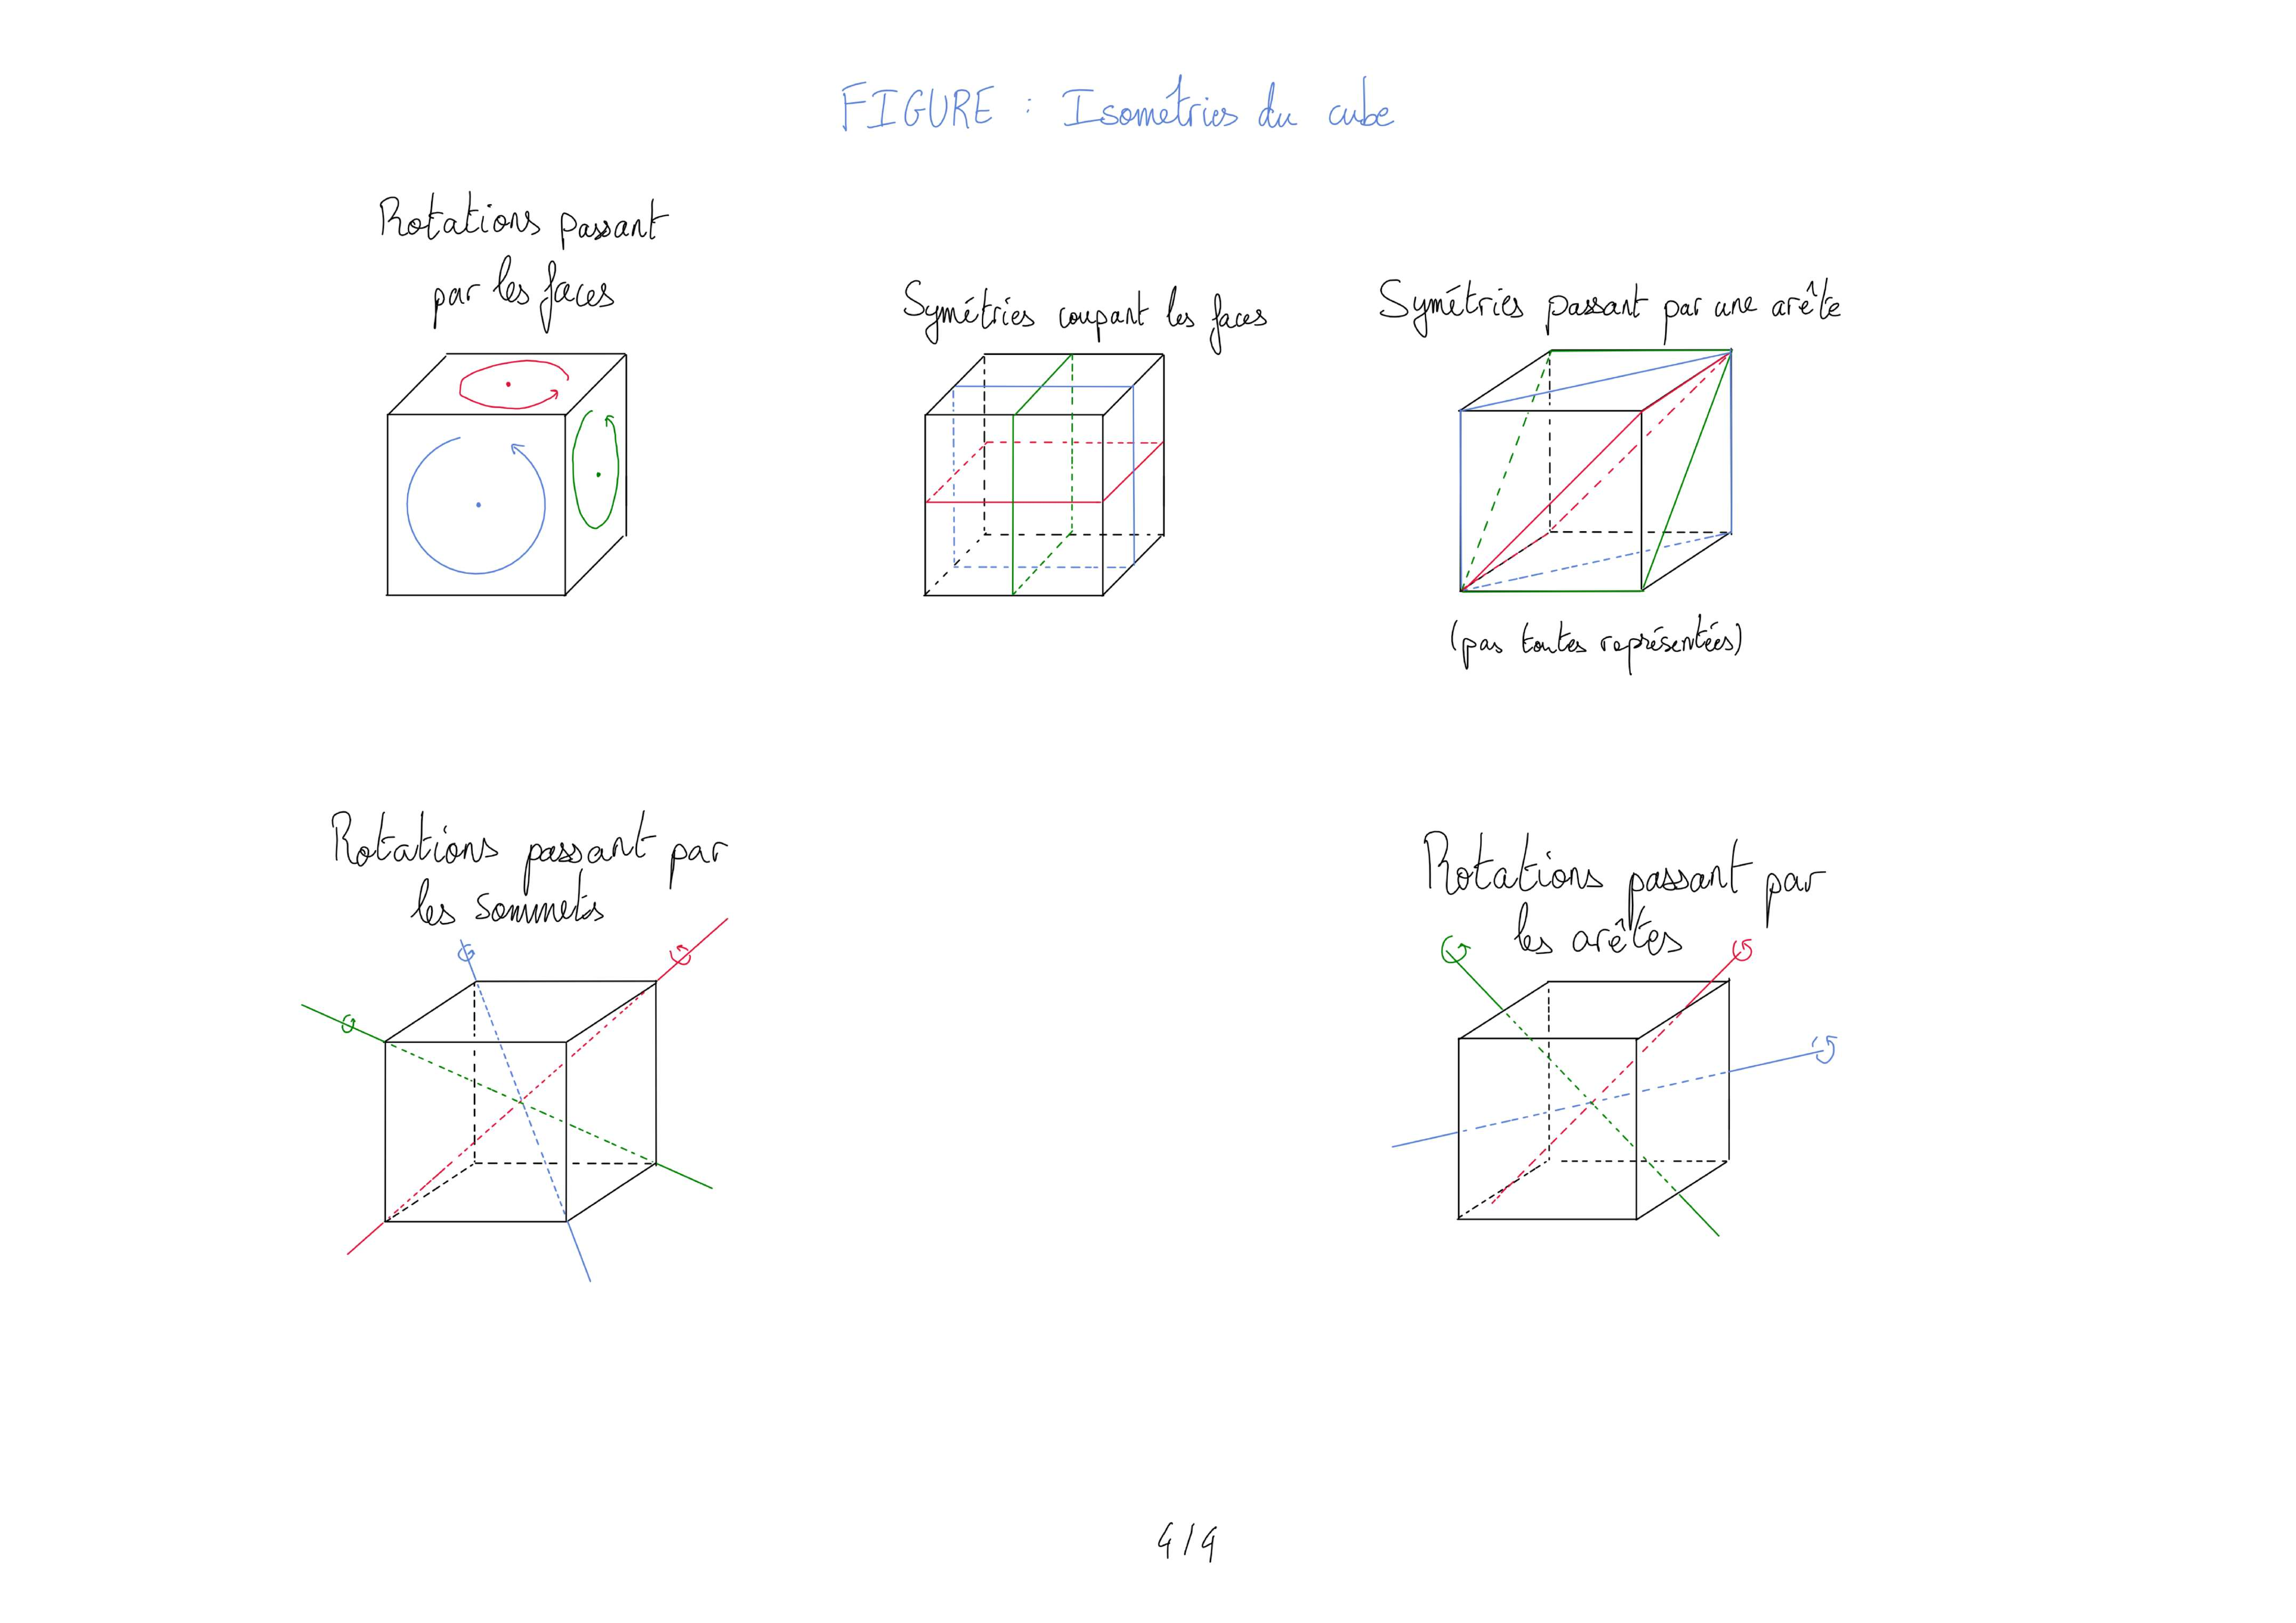
\includegraphics[trim={0 0 0 0},clip,width=1\linewidth]{img/101.pdf}
\end{figure}




\chapter*{102 : Groupe des nombres complexes de module 1. Racines de l'unité. Applications.}
\setcounter{definition}{0}
\section*{I. Les nombres complexes de module 1}
\begin{definition}
	L'ensemble des nombres complexes de module 1, aussi appelé \emph{cercle unité}, est noté $S^1:=\left\{z\in\IC\mid \vert z\vert = 1\right\}$.
\end{definition}

\subsection*{A. Autour de l'exponentielle}
\begin{definition}[\textnormal{[T] 43/44/45}]
	Pour $z\in\IC$, on définit :
	\begin{itemize}
		\item $\exp(z)=e^z = \sum_{n=0}^{+\infty} \frac{z^n}{n!}$ (l'\emph{exponentielle} de $z$)
		\item $\sin(z) = \sum_{n=0}^{+\infty} \frac{(-1)^n}{(2n+1)!}$ (le \emph{sinus} de $z$)
		\item $\cos(z) = \sum_{n=0}^{+\infty} \frac{(-1)^n}{(2n)!}$ (le \emph{cosinus} de $z$)
	\end{itemize}
\end{definition}

\begin{proposition}[\textnormal{[T] 43/35/44}]
	\begin{itemize}
		\item $\exp$, $\cos$ et $\sin$ sont des séries entières de rayon de convergence infini. En particulier, elles 
	sont entières. De plus, $\exp' = \exp$.
		\item $\forall\, z\in\IC,\, e^{iz}=\cos(z) + i\sin (z)$
		\item $\forall\, \theta\in\IR,\, \vert e^{i\theta}\vert=1$
	\end{itemize}
\end{proposition}

\begin{proposition}[\textnormal{[T] 44/44}]
	\begin{itemize}
		\item $\theta\mapsto e^{i\theta}$ est périodique. On note $\tau$ sa période. C'est un morphisme de groupes surjectif de $(\IR, +)$ dans $(S^1,\times)$.
		\item $\exp$ est un morphisme de groupes surjectif de $(\IC,+)$ dans $(\IC^*,\times)$. Son noyau est $i\tau\IZ$.
	\end{itemize}
\end{proposition}

\begin{definition}[\textnormal{[T] 44}]
	$\pi := \tau/2$. On admet que $\pi$ est transcendant sur $\IQ$.
\end{definition}

\begin{proposition}[\textnormal{[T] 45}]
	\begin{itemize}
		\item Formules d'Euler : $\forall\,z\in\IC,$ $\cos(z)=\frac{e^z +e^{-z}}{2}\in\IR$, $\sin(z)=\frac{e^z -e^{-z}}{2i}\in\IR$
		\item Formule de Moivre : $\forall \theta \in\IR,\,\forall n\in\IN,\, \left(e^{i\theta}\right)^n = e^{in\theta}$
	\end{itemize}
\end{proposition}

\begin{remark}[c.f. Figure 1]
	\begin{itemize}
		\item[$\vartriangleright$] La formule de Moivre est fausse pour $n$ non entier : 
	$1 = \left(e^{2i\pi}\right)^{1/2} \neq e^{i\pi} = -1$
		\item[$\vartriangleright$] $\cos^2 + \sin^2 = 1$
		\item[$\vartriangleright$] $\forall \theta\in\IR,\,\cos(\theta) = \Re(e^{i\theta})$ et $\sin(\theta) = \Im(e^{i\theta})$
	\end{itemize}
\end{remark}

\begin{application}
	Avec les formules de Moivre et d'Euler, pour tous $\theta\in\IR$ et $n\in\IN$, $\cos(n\theta)\in \IR[\cos(\theta)]$ et $\sin(n\theta)\in\IR[\sin(\theta)]$.

	(Appli : problème de trisection de l'angle - voir II. B)
\end{application}

\begin{application}[Polynômes de Techebychev]
	Ce sont les polynômes tels que $\forall n\in\IN,\, \forall\theta\in\IR,\, \cos(n\theta) = T_n(\theta)$
	et on a : $T_0 = 1$, $T_1 = X$, et $\forall n\in\IN,\, T_{n+2}=2XT_{n+1} - Tn$.
\end{application}

\begin{application}[Noyaux de Dirichlet et de Fejér]
	$\forall \theta \in\IR/2\pi\IZ,\, \forall n\in\IN^*,$
	$$D_N(\theta) := \sum_{n=-N}^{N} e^{in\theta}$$
	$$K_n(\theta) := \frac{1}{N}\sum_{n=0}^{N-1} D_N(\theta) = \left(\frac{\sin(N\theta/2)}{\sin(\theta/2)}\right)^2$$
\end{application}

\begin{theorem}[\textnormal{[R] 101}]\label{th:11}
	$\forall z\in S^1,\, \exists !\theta\in ]-\pi,\pi]\,\colon z = e^{i\theta}$
\end{theorem}

\begin{definition}[\textnormal{[R] 102}]
	Soit $z\in\IC^*$. D'après théorème \ref{th:11}, il existe un unique $\theta\in ]-\pi,\pi]$,
	appelé \emph{argument principal} de $z$, noté $\arg(z)$, tel que $z = \vert z \vert e^{i\theta}$.

	On appelle \emph{(un) argument} de $z$ tout réel $\theta$ tel que $z = \vert z \vert e^{i\theta}$. Les arguments de $z$ sont
	congrus à $\arg(z)$ modulo $2\pi$.
\end{definition}

\begin{definition}[\textnormal{[T] 63}]
	On appelle \emph{détermination principale du logarithme complexe} l'application :
	\begin{align*}
	\log : \IC\setminus \IR^- &\longrightarrow B_{\pi} := \left\{z\in\IC \mid |\Im(z)|<\pi\right\} \\
		z &\longmapsto \ln(|z|)+i\arg(z)
	\end{align*}
\end{definition}

\begin{proposition}
	$\exp$ induit une bijection de $B_{\pi}$ sur $\IC\setminus \IR^-$, de réciproque $\log$.
\end{proposition}

\begin{theorem}[de relèvement - ADMIS]
	Soit $I\subseteq \IR$ un intervalle et $k\in\IN$.
	Pour tout $f\in C^k(I,S^1)$, il existe $\varphi\in C^k(I,\IR)$ telle que $f = e^{i\varphi}$.
\end{theorem}

\subsection*{B. Les racines de l'unité}
\begin{definition}[\textnormal{[P] 80}]
	Soient $n\in\IN^*$ et $z\in\IC$.
	On dit que $z$ est une \emph{racine $n$-ième de l'unité} sir $z^n=1$. 
	On note $\IU_n$ l'ensemble des racines $n$-ièmes de l'unité.
	On dit que $z$ est une racine de l'unité sur $z\in \IU := \cup_{n\in\IN^*} \IU_n$.
\end{definition}

\begin{proposition}
	$\IU_n = \left\{e^{i\frac{2k\pi}{n}}\mid k\in \IN\right\} = \left\{e^{i\frac{2k\pi}{n}}\mid 0\leq k \leq n-1\right\} = \langle \omega_n \rangle$, 
	où $\omega_n := e^{i\frac{2\pi}{n}}$. En particulier, $\IU_n\cong \IZnZ$.
\end{proposition}

\begin{proposition}
	$\forall n\geq 2$, $\sum_{\omega\in\IU} \omega = 0$, $\omega^n = 1$, $\overline{\omega_n} = \omega_n^{n-1}$.
\end{proposition}

\begin{definition}[\textnormal{[P] 80}]
	Soit $n\in\IN^*$. On dit que $\zeta_n\in\IC$ est une \emph{racine primitive} $n$-ième de 
	l'unité si $\IU_n = \langle\zeta_n\rangle$. On note $\mu_n^*$ l'ensemble des racine primitives $n$-ièmes de l'unité, \emph{i.e.} des générateurs de $\IU_n$.
\end{definition}

\begin{proposition}[\textnormal{[P] 80}, cf FIGURE 2]
	$$\mu_n^* = \left\{\omega_n^k \mid k\wedge n = 1\right\}$$
\end{proposition}

\begin{example}
	$\IU_2 = \left\{\pm 1\right\}$, $\IU_3 = \left\{1,e^{2i\pi / 3},e^{-2i\pi/3}\right\} = \left\{1, \frac{1}{2} \pm i\frac{\sqrt{3}}{2}\right\}$, $\IU_4 = \left\{\pm 1, \pm i\right\}$.
\end{example}

\begin{proposition}[\textnormal{[P] 80, [Rb] 18}]
	Soit $(n,d)\in\left(\IN^*\right)^2$.
	\begin{itemize}
		\item[$\vartriangleright$] $\IU_d \subseteq \IU_n \iff d\mid n$
		\item[$\vartriangleright$] $\card \mu_n^* = \varphi(n)$ (indicatrice d'Euler)
		\item[$\vartriangleright$] $\IU_n = \sqcup_{d\mid n} \mu_d^*$
		\item[$\vartriangleright$] $n = \sum_{d\mid n} \varphi(d)$
	\end{itemize}
\end{proposition}

\begin{remark}
	Soient $a\in\IC^*$ et $n\in\IN^*$. Une racine $n$-ième de $a$ est un 
	nombre complexe $z$ vérifiant $z^n = a$. Posons $z_0 := |a|^{\frac{1}{n}}\exp(i\frac{\arg a}{n})$, de sorte que $z_0^n = a$.
	Si $z^n = a$, alors $\left(\frac{z}{z_0}\right)^n = 1$, \emph{i.e.} $\frac{z}{z_0}\in\IU_n$, donc 
	il existe $k\in\llbracket 0, n-1\rrbracket$ tel que $z = z_0e^{i\frac{2k\pi}{n}}$.
\end{remark}

\begin{theorem}[\textnormal{[Rb] 114/132}]
	Soit $H$ un sous-groupe de $S^1$. Si $H$ est fini d'ordre $n$, alors $H = \IU_n$. Sinon, $H$ est dense dans $S^1$.
\end{theorem}

\begin{application}[\textnormal{[Rb] 132}]
	$\overline{\left\{\cos (n) \mid n\in \IN\right\}} = \overline{\left\{\sin (n) \mid n\in \IN\right\}} = \left[0,1\right]$
\end{application}

\begin{theorem}[de Niven]
	Soit $r\in\IQ$. Si $\cos (r\pi)\in\IQ$, alors $r\in\left\{0, \frac{1}{3}, \frac{1}{2}\right\}$.
	Si $\sin(r\pi)\in\IQ$, alors $r\in\left\{0,\frac{1}{6}, \frac{1}{2}\right\}$.
\end{theorem}

\begin{corollary}
	$\IU\cap\IQ[i] = \left\{\pm 1, \pm i\right\}$
\end{corollary}

\subsection*{C. Polynômes cyclotomiques}
Soit $n\in \IN^*$.

\begin{definition}[\textnormal{[P] 80}]
	On appelle \emph{$n$-ième polynôme cyclotomique} le polynôme 
	$\Phi_n := \prod_{\zeta\in\mu_n^*} (X-\zeta)$.
\end{definition}

\begin{example}[\textnormal{[P] e81}]
	$\Phi_1 = X-1$, $\Phi_2 = X + 1$, $\Phi_3 = X^2 + X + 1$, $\Phi_4 = X^2 + 1$, ...
\end{example}

\begin{proposition}[\textnormal{[P] 80-83}]
	\begin{itemize}
		\item[$\vartriangleright$] $\deg(\Phi_n) = \varphi(n)$
		\item[$\vartriangleright$] $X^n - 1 = \prod_{d\mid n} \Phi_d$
		\item[$\vartriangleright$] $\Phi_n\in\IZ[X]$
		\item[$\vartriangleright$] $\Phi_n$ est irréductible sur $\IQ$
		\item[$\vartriangleright$] $\Phi_n$ est le polynôme minimal de $\zeta\in\mu_n^*$ sur $\IQ$
	\end{itemize}
\end{proposition}

\begin{proposition}
	Pour tout $p$ premier, 
	$$\Phi_p = \frac{X^p - 1}{X-1} = X^{p-1} + X^{p-2} + \dots + X + 1$$
\end{proposition}

\subsection*{D. Applications}

\begin{theorem}[de Wedderburn - \textnormal{[P] 82}]
	Tout corps fini est commutatif.
\end{theorem}

\begin{tcolorbox}[
    breakable, % Allows the theorem to split across pages
    colback=developpement, % The background color
    colframe=gray!0!black, % The frame color
    boxrule=0pt, % The frame thickness
    arc=1mm, % Sharp corners
	boxsep=0pt,
	left=0pt, right=0pt, top=0pt, bottom=0pt
]
\begin{theorem}[de Kronecker - \textnormal{[FGN] 213}]
	\label{dev11}
	Soit $P\in\IZ[X]$ unitaire dont toutes les racines sont de module $\leq 1$, et tel que 
	$P(0)\neq 0$. Alors toutes les racines de $P$ sont des racines primitives de l'unité.
\end{theorem}

\begin{corollary}[théorème de Kronecker - \textnormal{[Go] 95}]
	\label{dev12}
	Soit $P\in\IZ[X]$ irréductible sur $\IQ$. Si toutes les racines de $P$ sont 
	de module $\leq 1$, alors $P=X$ ou $P$ est cyclotomique.
\end{corollary}
\end{tcolorbox}

\section*{II. Liens avec la géométrie}
\subsection*{A. Notion d'angle orienté}
On note $S^1(0,1)$ le cercle unité de $\IR^2$ pour la norme euclidienne, qui s'identifie à 
$S^1$. Pour $z\in\IC$, on note $M_z$ le point de $\IR^2$ d'affixe $z$.

On note $\mathcal{B}$ une base orthonormée de $\IR^2$, que l'on décrète directe.

\begin{proposition}
	$\forall (\overrightarrow{u}, \overrightarrow{v}) \in S^1(0,1)^2,\, \exists ! r\in SO(\IR^2)\, : \overrightarrow{v} = r(\overrightarrow{u})$
\end{proposition}

\begin{theorem}[\textnormal{[P] 146}]
	On dispose des isomorphismes de groupes suivant :
	\begin{align*}
		\IR/2\pi\IZ &\longrightarrow S^1 &\longrightarrow &SO_2(\IR) &\longleftarrow &SO(\IR^2) \\
		\theta &\longmapsto e^{i\theta} &\longmapsto &R(\theta) &\longleftarrow &r_{\theta}
	\end{align*}

	NB : $R(\theta)$ est la matrice de rotation 2D d'angle $\theta$ (cos, -sin // sin, cos).
\end{theorem}

\begin{corollary}
	La relation $\left(\overrightarrow{u},\overrightarrow{v}\right)\mathcal{R}\left(\overrightarrow{u'},\overrightarrow{v'}\right) \iff \exists r\in SO(\IR^2)\,\colon \overrightarrow{u'} = r(\overrightarrow{u})$ et $\overrightarrow{v'}=r(\overrightarrow{v})$
	est une relation d'équivalence sur $\left(S^1\right)^2$.
\end{corollary}

\begin{definition}[\textnormal{[P] 146} - FIGURE 3]
	Soit $\left(\overrightarrow{u},\overrightarrow{v}\right)\in\left(S^2\right)^2$.
	\begin{itemize}
		\item[$\vartriangleright$] On appelle \emph{angle orienté de $\overrightarrow{u}$ à $\overrightarrow{v}$} la classe d'équivalence de $\left(\overrightarrow{u},\overrightarrow{v}\right)$ dans $\left(S^1\right)^2/\mathcal{R}$, que l'on note $\widehat{(\overrightarrow{u}, \overrightarrow{v})}$.
		\item[$\vartriangleright$] Une \emph{mesure} de $\widehat{(\overrightarrow{u}, \overrightarrow{v})}$ est un réel $\theta$ tel que $\overrightarrow{v} = r_{\theta}(\overrightarrow{u})$.
		\item[$\vartriangleright$] La \emph{mesure principale} de $\widehat{(\overrightarrow{u}, \overrightarrow{v})}$ est la mesure de $\widehat{(\overrightarrow{u}, \overrightarrow{v})}$ entre $-\pi$ et $\pi$.
	\end{itemize}
\end{definition}

\begin{definition}
	On étend la définition aux couples de vecteurs non nuls $\left(\overrightarrow{u},\overrightarrow{v}\right)$ en posant :
	$$\widehat{\left(\overrightarrow{u},\overrightarrow{v}\right)} := \widehat{\left(\frac{\overrightarrow{u}}{\|\overrightarrow{u}\|},\frac{\overrightarrow{v}}{\|\overrightarrow{v}\|}\right)}$$
\end{definition}

\begin{remark}
	Si $z_{\overrightarrow{u}}$ est l'affixe de $\overrightarrow{u}\in\IR^2$, alors l'affixe de $r_{\theta}(\overrightarrow{u})$ est $e^{i\theta}z_{\overrightarrow{u}}$.
\end{remark}

\begin{remark}
	En notant $\langle\cdot \mid \cdot \rangle$ le produit scalaire euclidien de $\IR^2$, on appelle \emph{écart angulaire} entre 
	deux vecteurs non nuls $\overrightarrow{u}$ et $\overrightarrow{v}$ le réel $\alpha= \arccos\left(\frac{\langle\overrightarrow{u}\mid\overrightarrow{v}\rangle}{\|\overrightarrow{u}\|\cdot\|\overrightarrow{v}\|}\right)$.
	Si $\theta$ est la mesure principale de $\widehat{(\overrightarrow{u}, \overrightarrow{v})}$, alors $\alpha = |\theta |$.

	Plus précisement, si $\overrightarrow{u}$ et $\overrightarrow{v}$ sont colinéaires et de même sens (resp. de sens opposé), alors $\alpha = \theta = 0$ 
	(resp. $\alpha = \theta = \pi$) et sinon, si $\widehat{(\overrightarrow{u}, \overrightarrow{v})}$ est directe, alors $\alpha = \theta$ et sinon $\alpha = -\theta$.
\end{remark}

\begin{proposition}[\textnormal{[Bu] 497}]
	Une mesure de $\widehat{(\overrightarrow{u},\overrightarrow{v})}$ est un réel $\theta$ vérifiant 
	$$e^{i\theta} = \frac{\langle\overrightarrow{u}\mid \overrightarrow{v}\rangle + i\det_{\mathcal{B}}(\overrightarrow{u},\overrightarrow{v})}{\|\overrightarrow{u}\|\cdot\|\overrightarrow{v}\|}$$
\end{proposition}

\begin{definition}
	Soient $\overrightarrow{u}$ et $\overrightarrow{v}$ deux vecteurs non nuls d'écart angulaire $\alpha$.
	On dit que $\widehat{(\overrightarrow{u},\overrightarrow{v})}$ est \emph{nul} si $\alpha = 0$, \emph{plat} si $\alpha = \pi$, \emph{droit} si $\alpha = \pi/2$, \emph{aigu} si $\alpha < \pi/2$ et \emph{obtus} si $\alpha > \pi/2$.
\end{definition}

\subsection*{B. Autour des polygônes réguliers - groupes diédraux, constructibilité}
Soit $n \geq 3$.
\begin{definition}
	Le \emph{polygône régulier à $n$ côtés} est le polygône convexe $P_n$ du plan dont les sommets sont, dans l'ordre, les points d'affixes $1, \omega_n,\omega_n^2,\dots,\omega_n^{n-1}$.
\end{definition}
\begin{proposition}
	L'ensemble des isométries du plan conservant $P_n$ est un groupe, appelé \emph{groupe diédral d'ordre $2n$} et noté $D_{2n}$.
	Il est engendré par la rotation d'angle $\frac{2\pi}{n}$ centrée à l'origine (correspondant à $z\mapsto \omega_nz$ en termes d'affixes) et la symétrie d'axe $(Ox)$ (correspondant à la conjugaison en termes d'affixes).
\end{proposition}

\begin{definition}[\textnormal{[P] 68}]
	On dit que $z\in\IC$ est \emph{constructible} si on peut tracer l'image de $z$ dans le plan uniquement avec un compas et une règle non graduée.
	On dit que $P_n$ est constructible si $\omega_n$ l'est.
\end{definition}

\begin{theorem}[de Gauss-Wantzel - FIGURES 2,4]
	$P_n$ est constructible si, et seulement si, $n$ est de la forme $n=2^m p_1\dots p_r$, avec $m\in \IN$ et $p_1, \dots, p_r$ des nombres premiers de Fermat (\emph{i.e.} $3,5,17,257, 65537$).
\end{theorem}

\subsection*{C. Application : une caractérisation de $7$}

\begin{tcolorbox}[
    breakable, % Allows the theorem to split across pages
    colback=developpement, % The background color
    colframe=gray!0!black, % The frame color
    boxrule=0pt, % The frame thickness
    arc=1mm, % Sharp corners
	boxsep=0pt,
	left=0pt, right=0pt, top=0pt, bottom=0pt
]
\begin{theorem}[de Gauss-Lucas - \textnormal{[FGN] 225}]
	\label{102dev21}
	Soit $P\in\IC[X]$ non constant.
	$$Z-{\IC}(P')\subset \text{Conv}(Z_{\IC}(P))$$
	où, si $Z_{\IC}(P) = \left\{\alpha_1,\dots,\alpha_r\right\}$, alors :
	$$\text{Conv}(Z_{\IC}(P)) = \left\{\sum_{k=1}^{r}\lambda_k\alpha_k \mid (\lambda_1,\dots,\lambda_r)\in \left[0,1\right]^r,\, \sum_{k=1}^{r}\lambda_k = 1\right\}$$
\end{theorem}

\begin{application}
	\label{102dev22}
	$7$ est le plus grand entier $n\geq 2$ tel que :
	$$Z_{\IC}((X+1)^n - X^n - 1)\subseteq \left\{z\in \IC \mid |z| = 1\right\}$$
\end{application}
\end{tcolorbox}

\section*{Développements}
\begin{itemize}
	\item Développement 1 : Théorème \ref{dev11} et Corrolaire \ref{dev12}
	\item Développement 2 : Théorème \ref{102dev21} et Application \ref{102dev22}
\end{itemize}

\section*{Références}
\begin{itemize}
	\item[Rb] \emph{Mathématiques pour l'agrégation - Algèbre et géométrie}, Jean-Étienne Rombaldi, 2e édition
	\item[Rb] \emph{Eléments d'analyse réelle}, Rombaldi
	\item[P] Perrin
	\item[FGN] \emph{Oraux X-ENS, Algèbre 1}, 2è édition (Francinou)
	\item[T] \emph{Analyse complexe}, Tauvel
	\item[Bu] Burg
\end{itemize}

\chapter*{105 : Groupe des permutations d'un ensemble fini. Applications.}
\setcounter{definition}{0}
\section*{I. Permutations d'un ensemble fini}
\subsection*{A. Introduction}
\begin{definition}[\textnormal{[R] 37}]
	Soit $E$ un ensemble. On note $\mathfrak{S}(E)$
	l'ensemble des bijections de $E$ dans $E$. On l'appelle \emph{groupe symétrique} de $E$.
	On notera plus simplement $\mathfrak{S}_n = \mathfrak{S}(\llbracket 1, n\rrbracket)$.
	On appelle \emph{permutation} de $E$ un élément de $\mathfrak{S}(E)$.
\end{definition}

\begin{proposition}
	$\mathfrak{S}(E)$ est un groupe pour la composition, de neutre l'identité de $E$.
\end{proposition}

\begin{proposition}[\textnormal{[R] 39}]
	Si $E$ et $F$ sont deux ensembles équipotents, alors $\mathfrak{S}(E)$ et $\mathfrak{S}(F)$ sont isomorphes (en tant que groupes).
\end{proposition}

\begin{proposition}[\textnormal{[R] 39}]
	Pour $n\geq 3$, $\mathfrak{S}_3$ n'est pas commutatif.
\end{proposition}

Dans toute la suite, on étudiera $\mathfrak{S}_n$ pour $n\geq 3$.

\begin{proposition}[\textnormal{[R] 40}]
	$\#\mathfrak{S}_n = n!$
\end{proposition}

\begin{notation*}[\textnormal{[U] 41}]
	Soit $\sigma\in\mathfrak{S}_n$. On représentera $\sigma$ par la matrice $2\times n$ :
	\begin{align*}
		\sigma = \left(\begin{smallmatrix} 
			1 & 2 & \cdots & n\\
			\sigma(1) & \sigma(2) & \cdots & \sigma(n)
		\end{smallmatrix}\right)
	\end{align*}
\end{notation*}

\subsection*{B. Action naturelle de $\mathfrak{S}_n$ sur $\llbracket 1,n\rrbracket$, conséquences}

\begin{proposition}[\textnormal{[U] 41}]
		$\mathfrak{S}_n$ agit naturellement sur $\llbracket 1,n\rrbracket$ par $\sigma \cdot i = \sigma(i)$.
		Le morphisme associé est l'identité de $\mathfrak{S}_n$.
\end{proposition}

\begin{definition}[\textnormal{[U] 42}]
	On note $\Fix(\sigma)$ l'ensemble des points fixes de $\sigma\in\mathfrak{S}_n$.
	Son complémentaire dans $\llbracket 1,n\rrbracket$ est appelé \emph{support} de $\sigma$, et est noté $\Supp(\sigma)$.
\end{definition}

\begin{proposition}[\textnormal{[U] 43}]
	Soit $\sigma \in \mathfrak{S}_n$. Le sous-groupe $\langle\sigma\rangle$ agit sur $\llbracket 1,n\rrbracket$ par restriction
	de l'action de $\mathfrak{S}_n$. Les orbites de cette action sont appelées \emph{$\sigma$-orbites}.
	La réunion des $\sigma$-orbites ponctuelles est $\Fix(\sigma)$. Les $\sigma$-orbites non ponctuelles partitionnent $\Supp(\sigma)$.
\end{proposition}

\begin{example}
	Soit $\sigma = \left(\begin{smallmatrix} 
			1 & 2 & 3 & 4 & 5 \\
			2 & 1 & 3 & 5 & 4
		\end{smallmatrix}\right)$.
	On a $\Supp(\sigma)=\left\{1,2\right\}\sqcup \left\{4,5\right\}=\langle\sigma\rangle\cdot \left\{1\right\}\sqcup \langle\sigma\rangle\cdot\left\{4\right\}$.
\end{example}

\begin{definition}[\textnormal{[U] 43}]
	Un \emph{$k$-cycle} ($2\leq k \leq n$) est une permutation n'ayant qu'une seule $\sigma$-orbite non ponctuelle $\left\{i_1,\dots,i_k\right\}$.
	On la note $\sigma = (i_1,\dots,i_k)$ pour signifier que 
	$\forall j\notin \left\{i_1,\dots,i_k\right\}$, $\sigma(j)=j$ et $\sigma(i_j)=i_{j+1}$ en regardant les indices modulo $k$.

	Un $2$-cycle est appelé \emph{transposition}.
\end{definition}

\begin{proposition}[\textnormal{[U] 43}]
	$(i_1,i_2,\dots,i_k) = (i_2,i_3,\dots,i_k,i_1)=\dots=(i_k,i_1,i_2,\dots,i_{k-1})$
\end{proposition}

\begin{proposition}
	Un $k$-cycle est d'ordre $k$.
\end{proposition}

\subsection*{C. Décomposition d'une permutation, conséquences}

\begin{proposition}[\textnormal{[U] 42}]
	Deux permutations à supports disjoints commutent.
\end{proposition}

\begin{theorem}[\textnormal{[U] 43}]
	Toute permutation se décompose de manière unique (à l'ordre des facteurs près) comme produit de cycles à supports disjoints.
\end{theorem}

\begin{algorithm}[\textnormal{[U] 43}]
	Pour trouver une telle décomposition, il suffit de trouver les $r$-orbites.
	\begin{enumerate}
		\item On calcule $\sigma(1), \sigma^2(1),\dots$ justqu'à trouver $\sigma^{k_1}(1)=1$ (NB : $k_1\leq n$) ;
		\item On pose $i_2 = \min \llbracket 1,n\rrbracket \setminus (\langle\sigma\rangle\cdot\left\{1\right\})$, et de même on calcule $\sigma(i_2),\sigma^2(i_2),\dots$ jusqu'à trouver $\sigma^{k_2}(i_2)=i_2$ ;
		\item On itère jusqu'à épuiser $\llbracket 1,n\rrbracket$.
	\end{enumerate}
	On a alors $\sigma = (1,\sigma(1),\dots,\sigma^{k_1-1}(1))\circ (i_2, \sigma(i_2),\dots,\sigma^{k_2-1}(i_2))\circ \dots \circ(i_j, \sigma(i_j),\dots,\sigma^{k_j-1}(i_j))$
\end{algorithm}

\begin{example}
	$\sigma = \left(\begin{smallmatrix} 
			1 & 2 & 3 & 4 & 5 & 6 \\
			3 & 2 & 4 & 1 & 6 & 5
		\end{smallmatrix}\right) = (1,3,4)(5,6)$
\end{example}

\begin{proposition}[\textnormal{[R] 44}]
		$(i_1,\dots,i_k) = (i_1,i_2)(i_2,i_3)\dots(i_{k-1},i_k)$
\end{proposition}
\begin{corollary}[\textnormal{[R] 44}]
	Les transpositions engendrent $\mathfrak{S}_n$.
\end{corollary}
\begin{proposition}[\textnormal{[R] 45}]
	$\mathfrak{S}_n = \langle(i,i+1),\, 1\leq i\leq n\rangle = \langle (1,i), \, 2\leq i \leq n\rangle = \langle(1,2),\, (1,2,\dots, n) \rangle$
\end{proposition}

\begin{definition}[\textnormal{[U] 45}]
	On appelle \emph{type} de $\sigma\in\mathfrak{S}_n$ la liste croissante des cardinaux des $\sigma$-orbites.
\end{definition}

\begin{example}
	Le type de $(1,2,5)(3,4)(7,8)\in\mathfrak{S}_8$ est la liste $\left[1,2,2,3\right]$.
\end{example}

\begin{proposition}[\textnormal{[U] 46}]
	Deux permutations sont conjuguées dans $\mathfrak{S}_n$ si, et seulement si, elles ont le même type.
	Cela décrit donc les classes de conjugaison de $\mathfrak{S}_n$.
\end{proposition}

\begin{proposition}[\textnormal{[U] 45}]
	Si $\sigma$ est du type $\left[l_1,\dots,l_k\right]$, alors $\ord(\sigma) = l_1 \vee \dots \vee l_k$.
\end{proposition}

\subsection*{D. Signature dune permutation, groupe alterné}

\begin{proposition}[\textnormal{[R] 47}]
	Il existe un unique morphisme $\varepsilon\,\colon \mathfrak{S}_n \to \left\{\pm 1\right\}$ qui envoie
	les transpositions sur $-1$. On appelle \emph{signature} de $\sigma$ la quantité $\varepsilon(\sigma)$.
\end{proposition}

\begin{corollary}
	La signature d'un $k$-cycle est $(-1)^{k+1}$.
\end{corollary}

\begin{proposition}[\textnormal{[R] 48}]
	$\forall\sigma\in\mathfrak{S}_n$, 
	$$\varepsilon(\sigma) = \prod_{1\leq i\leq j\leq n}\frac{\sigma(j) - \sigma(i)}{j-i}$$
	En particulier, la signature mesure le nombre d'inversions.
\end{proposition}

\begin{definition}[\textnormal{[R] 48}]
	On appelle \emph{$n$-ième groupe alterné} le sous-groupe $\mathcal{A}_n = \Ker(\varepsilon)$.
	C'est l'ensemble des permutations dîtes \emph{paires}.
\end{definition}

\begin{example}
	$\mathcal{A}_3 = \left\{\textnormal{id},\, (1,2,3),\, (1,3,2)\right\}$.
\end{example}

\begin{proposition}
	$\#\mathcal{A}_n = \frac{n!}{2}$
\end{proposition}

\begin{theorem}[\textnormal{[R] 49}]
	Pour $n\geq 3$, les $3$-cycles engendrent $\mathcal{A}_n$, et y sont conjugués.
\end{theorem}

\begin{theorem}[\textnormal{[R] 50}]
	Pour $n\geq 5$, $\mathcal{A}_n$ n'admet pas de sous-groupe distingué non trivial.
\end{theorem}

\section*{II. Quelques applications du groupe symétrique}
\subsection*{A. En géométrie : les isométries des polytopes}

\begin{theorem}[\textnormal{[R] 94}]
	L'ensemble des isométries du plan conservant un triangle équilatéral est un groupe isomorphe à $\mathfrak{S}_3$.
\end{theorem}

\begin{proposition}[\textnormal{[R] 82}]
	Soit $\mathcal{C}$ un cube. L'ensemble des isométries de l'espace conservant $\mathcal{C}$ est un groupe, noté $\Is(\mathcal{C})$.
	On note $\Is^+(\mathcal{C})$ le sous-groupe de $\Is(\mathcal{C})$ formé des rotations.
\end{proposition}

\begin{tcolorbox}[
    breakable, % Allows the theorem to split across pages
    colback=developpement, % The background color
    colframe=gray!0!black, % The frame color
    boxrule=0pt, % The frame thickness
    arc=1mm, % Sharp corners
	boxsep=0pt,
	left=0pt, right=0pt, top=0pt, bottom=0pt
]
\begin{theorem}[\textnormal{[R] 85}]
	\label{105dev1}
	$\Is^+(\mathcal{C}) \cong \mathfrak{S}_4$ et $\Is(\mathcal{C})\cong \mathfrak{S}_4\times \IZ/2\IZ$.
\end{theorem}
\end{tcolorbox}

\begin{theorem}[\textnormal{[R] 95}]
	En notant $\mathcal{T}$ le tétraèdre régulier, on a :
	$\Is(\mathcal{T})\cong \mathfrak{S}_4$ et $\Is^+(\mathcal{T})\cong \mathcal{A}_4$.
\end{theorem}

\subsection*{Chez les (actions de) groupes}
\begin{theorem}[de Cayley - \textnormal{[R] 53}]
	Tout groupe fini d'ordre $n$ est isomorphe à un sous-groupe de $\mathfrak{S}_n$.
\end{theorem}
\begin{proposition}
	Comme pout tout corps (commutatif) $K$, $\mathfrak{S}_n\actson GL_n(K)$, tout groupe de garde $n$ 
	est isomorphe à un sous-groupe de $GL_n(K)$.
\end{proposition}

\begin{example}
	Soit $D_{2\times 4}$ le groupe des isométries du carré. Comme $\#D_{2\times 4} = 8$, $D_{2\times 4}$ est isomorphe à un sous-groupe de $\mathfrak{S}_8$. Noton $\varphi$ un tel isomorphisme.
	Comme $D_{2\times 4} = \langle r, s\rangle$ où $\ord(r) = 4$, $\ord(s) = 2$ et $\ord(rs) = 2$, on a $\varepsilon\circ \varphi(s)=\varepsilon\circ \varphi(rs) = -1$, donc $\varepsilon\circ \varphi(r) = 1$.
\end{example}

\subsection*{C. Polynômes symétriques}
\begin{definition}[\textnormal{[R] 55}]
	Un \emph{polynôme symétrique} est un polynôme $P\in K[X_1,\dots,X_n]$
	tel que $\forall\sigma\in\mathfrak{S}_n$, $P(X_{\sigma(1)},\dots,X_{\sigma(n)}) = P(X_1,\dots,X_n)$.
\end{definition}

\begin{definition}[\textnormal{[R] 55}]
	Les \emph{polynômes symétriques élémentaires} sont les 
	\begin{align*}
		\Sigma_{k,n} = \sum_{1\leq i_1\leq\dots\leq i_k\leq n} X_{i_1}\dots X_{i_k}\in K[X_1,\dots,X_n]
	\end{align*}
\end{definition}

\begin{theorem}[ADMIS - \textnormal{[R] 55}]
	Pour tout polynôme symétrique $P\in K[X_1,\dots,X_n]$, il
	existe un unique polynôme $Q\in K[X_1,\dots,X_n]$ tel que 
	$P(X_1,\dots,X_n) = Q(\Sigma_{1,n},\dots,\Sigma_{n,n})$.
\end{theorem}

\subsection*{D. En algèbre (multi-)linéaire}
Dans ce paragraphe, $E$ est un $\mathbb{K}$-espace vectoriel de dimension finie $n$.
On fixe une base $\mathcal{B} = (e_1,\dots,e_n)$ de $E$.
\begin{definition}[\textnormal{[R] 545}]
	Une \emph{forme $k$-linéaire} sur $E$ est une application $\varphi \,\colon E^k\to \mathbb{K}$ telle que pour tout $i\in\llbracket 1,n\rrbracket$, pour tout $(x_1,\dots, x_k)\in E^k$,
	$\varphi(x_1,\dots,x_{i-1}, \cdot, x_{i+1}, \dots, x_k)$ est linéaire.

	On note $\bigotimes^k E^*$ l'ensemble des formes $k$-linéaires sur $E$.
\end{definition}

\begin{proposition}[\textnormal{[R] 546}]
	$\left(e_{i_1}^*\otimes\dots\otimes e_{i_k}^*\right)_{1\leq i_1<\dots < i_k\leq n}$ est une base de $\bigotimes^kE^*$,
	où pour $(x_1,\dots, x_k)\in E^k$, $e_{i_1}^*\otimes\dots\otimes e_{i_k}^*(x_1,\dots, x_k) = e_{i_1}^*(x_1)\dots e_{i_k}^*(x_k)$.
\end{proposition}

\begin{definition}[\textnormal{[R] 546}]
	Une forme $k$-linéaire \emph{alternée} est une forme $k$-linéaire $\varphi\in\bigotimes^kE^*$
	telle que $\forall\sigma\in\mathfrak{S}_k$, $\forall(x_1,\dots, x_k)\in E^k$, $\varphi(x_{\sigma(1)},\dots, x_{\sigma(k)}) = \varepsilon(\sigma)\varphi(x_1,\dots, x_k)$.

	On note $\bigwedge^k E^*$ l'espace des formes $k$-linéaires alternées sur $E$.
\end{definition}

\begin{proposition}
	$\left(e_{i_1}^*\wedge \dots \wedge e_{i_k}^*\right)_{1\leq i_1 < \dots < i_k\leq n}$ est une base de $\bigwedge^kE^*$, où pour $(x_1,\dots,x_k)\in E^k$,
	$e_{i_1}^*\wedge \dots \wedge e_{i_k}^*(x_1,\dots,x_k) = \sum_{\sigma\in\mathfrak{S}_k} \varepsilon(\sigma) e_{i_1}^*(x_{\sigma(1)}) \dots e_{i_k}^*(x_{\sigma(k)})$.
\end{proposition}

\begin{corollary}
	On a $\dim\left(\bigwedge^kE^*\right) = {n \choose k}$.
\end{corollary}

\begin{definition}
	On appelle \emph{déterminant dans la base $\mathcal{B}$} l'unique forme $n$-linéaire alternée $\det_{\mathcal{B}}$ sur $E$ vérifiant
	$\det_{\mathcal{B}}(\mathcal{B}) = 1$. (La fammille $\left(\det_{\mathcal{B}}\right)$ est une base de $\bigwedge^n E^*$.)
\end{definition}

\begin{proposition}[\textnormal{[R] 547}]
	$\forall(x_1,\dots, x_n)\in E^n$, $\det_{\mathcal{B}}(x_1,\dots,x_n) = \sum_{\sigma\in\mathfrak{S}_n} \varepsilon(\sigma)e_1^*(x_{\sigma(1)})\dots e_n^*(x_{\sigma(n)})$.
\end{proposition}

\subsection*{E. Résultats en probabilités}

\begin{definition}[\textnormal{[R] 51}]
	On appelle \emph{dérangement} une permutation sans point fixes.
\end{definition}

\begin{proposition}
	Notons $d_n$ le nombre de dérangements de $\llbracket 1,n\rrbracket$.
	Alors $d_n = n!\sum_{k=0}^{n}\frac{(-1)^k}{k!}$. En particulier, la probabilité
	de choisir un dérangement en tiant au hasard une permutation de $\llbracket 1,n\rrbracket$ tend vers $\frac{1}{e}$ quand $n\to +\infty$.
\end{proposition}

\begin{proposition}[\textnormal{[C]}]
	Soit $X$ la variable aléatoire qui compte le nombre de points fixes d'une permutation aléatoirement choisie dans $\mathfrak{S}_n$.
	Alors $\mathbb{E}[X] = \mathbb{V}[X] = 1$.
\end{proposition}

\subsection*{F. Groupes simples d'ordre 60}
Dans ce paragraphe, on se donne $p$ premier, et on note $\#G = p^{\alpha}m$, $m\wedge p = 1$.

\begin{definition}[\textnormal{[U] 85}]
	Un \emph{$p$-Sylow} de $G$ est un sous-groupe de $G$ de cardinal $p^{\alpha}$.
\end{definition}

\begin{notation*}
	$\Syl_p(G)$ désigne l'ensemble des $p$-Sylow de $G$, et $n_p =\#\Syl_p(G)$.
\end{notation*}

\begin{theorem}[de Sylow - \textnormal{[U] 87}]
	Soit $G$ un groupe d'ordre $p^{\alpha}m$, $p$ premier et $m\wedge p = 1$.
	\begin{enumerate}
		\item $\Syl_p(G)\neq \emptyset$
		\item $G$ agit transitivement sur $\Syl_p(G)$ par conjugaison
		\item $n_p \equiv 1\,[p]$ (donc $n_p\mid m$).
	\end{enumerate}
\end{theorem}

\begin{definition}
	On dit que $G$ est \emph{simple} si les seuls sous-groupes de $G$ distingués (\emph{i.e.} fixe par l'action par conjugaison de G) sont $\left\{1\right\}$ et $G$.
\end{definition}

\begin{tcolorbox}[
    breakable, % Allows the theorem to split across pages
    colback=developpement, % The background color
    colframe=gray!0!black, % The frame color
    boxrule=0pt, % The frame thickness
    arc=1mm, % Sharp corners
	boxsep=0pt,
	left=0pt, right=0pt, top=0pt, bottom=0pt
]
\begin{theorem}[\textnormal{[S] - 277}]
	\label{105dev2}
	Si $G$ est simple et d'ordre $60$, alors $G\cong \mathcal{A}_5$.
\end{theorem}
\end{tcolorbox}

\section*{Développements}
\begin{itemize}
	\item Développement 1 : Théorème \ref{105dev1}
	\item Développement 2 : Théorème \ref{105dev2}
\end{itemize}

\section*{Références}
\begin{itemize}
	\item[R] \emph{Mathématiques pour l'agrégation - Algèbre et géométrie}, Jean-Étienne Rombaldi, 2e édition
	\item[U] \emph{Théorie des groupes}, Félix Ulmer
	\item[S] \emph{Algèbre pour la licence 3}, Szpirglas
	\item[C] \emph{Carnets de voyage en Algébrie}, Caldero
\end{itemize}

\begin{figure}[!htb]
	\centering
	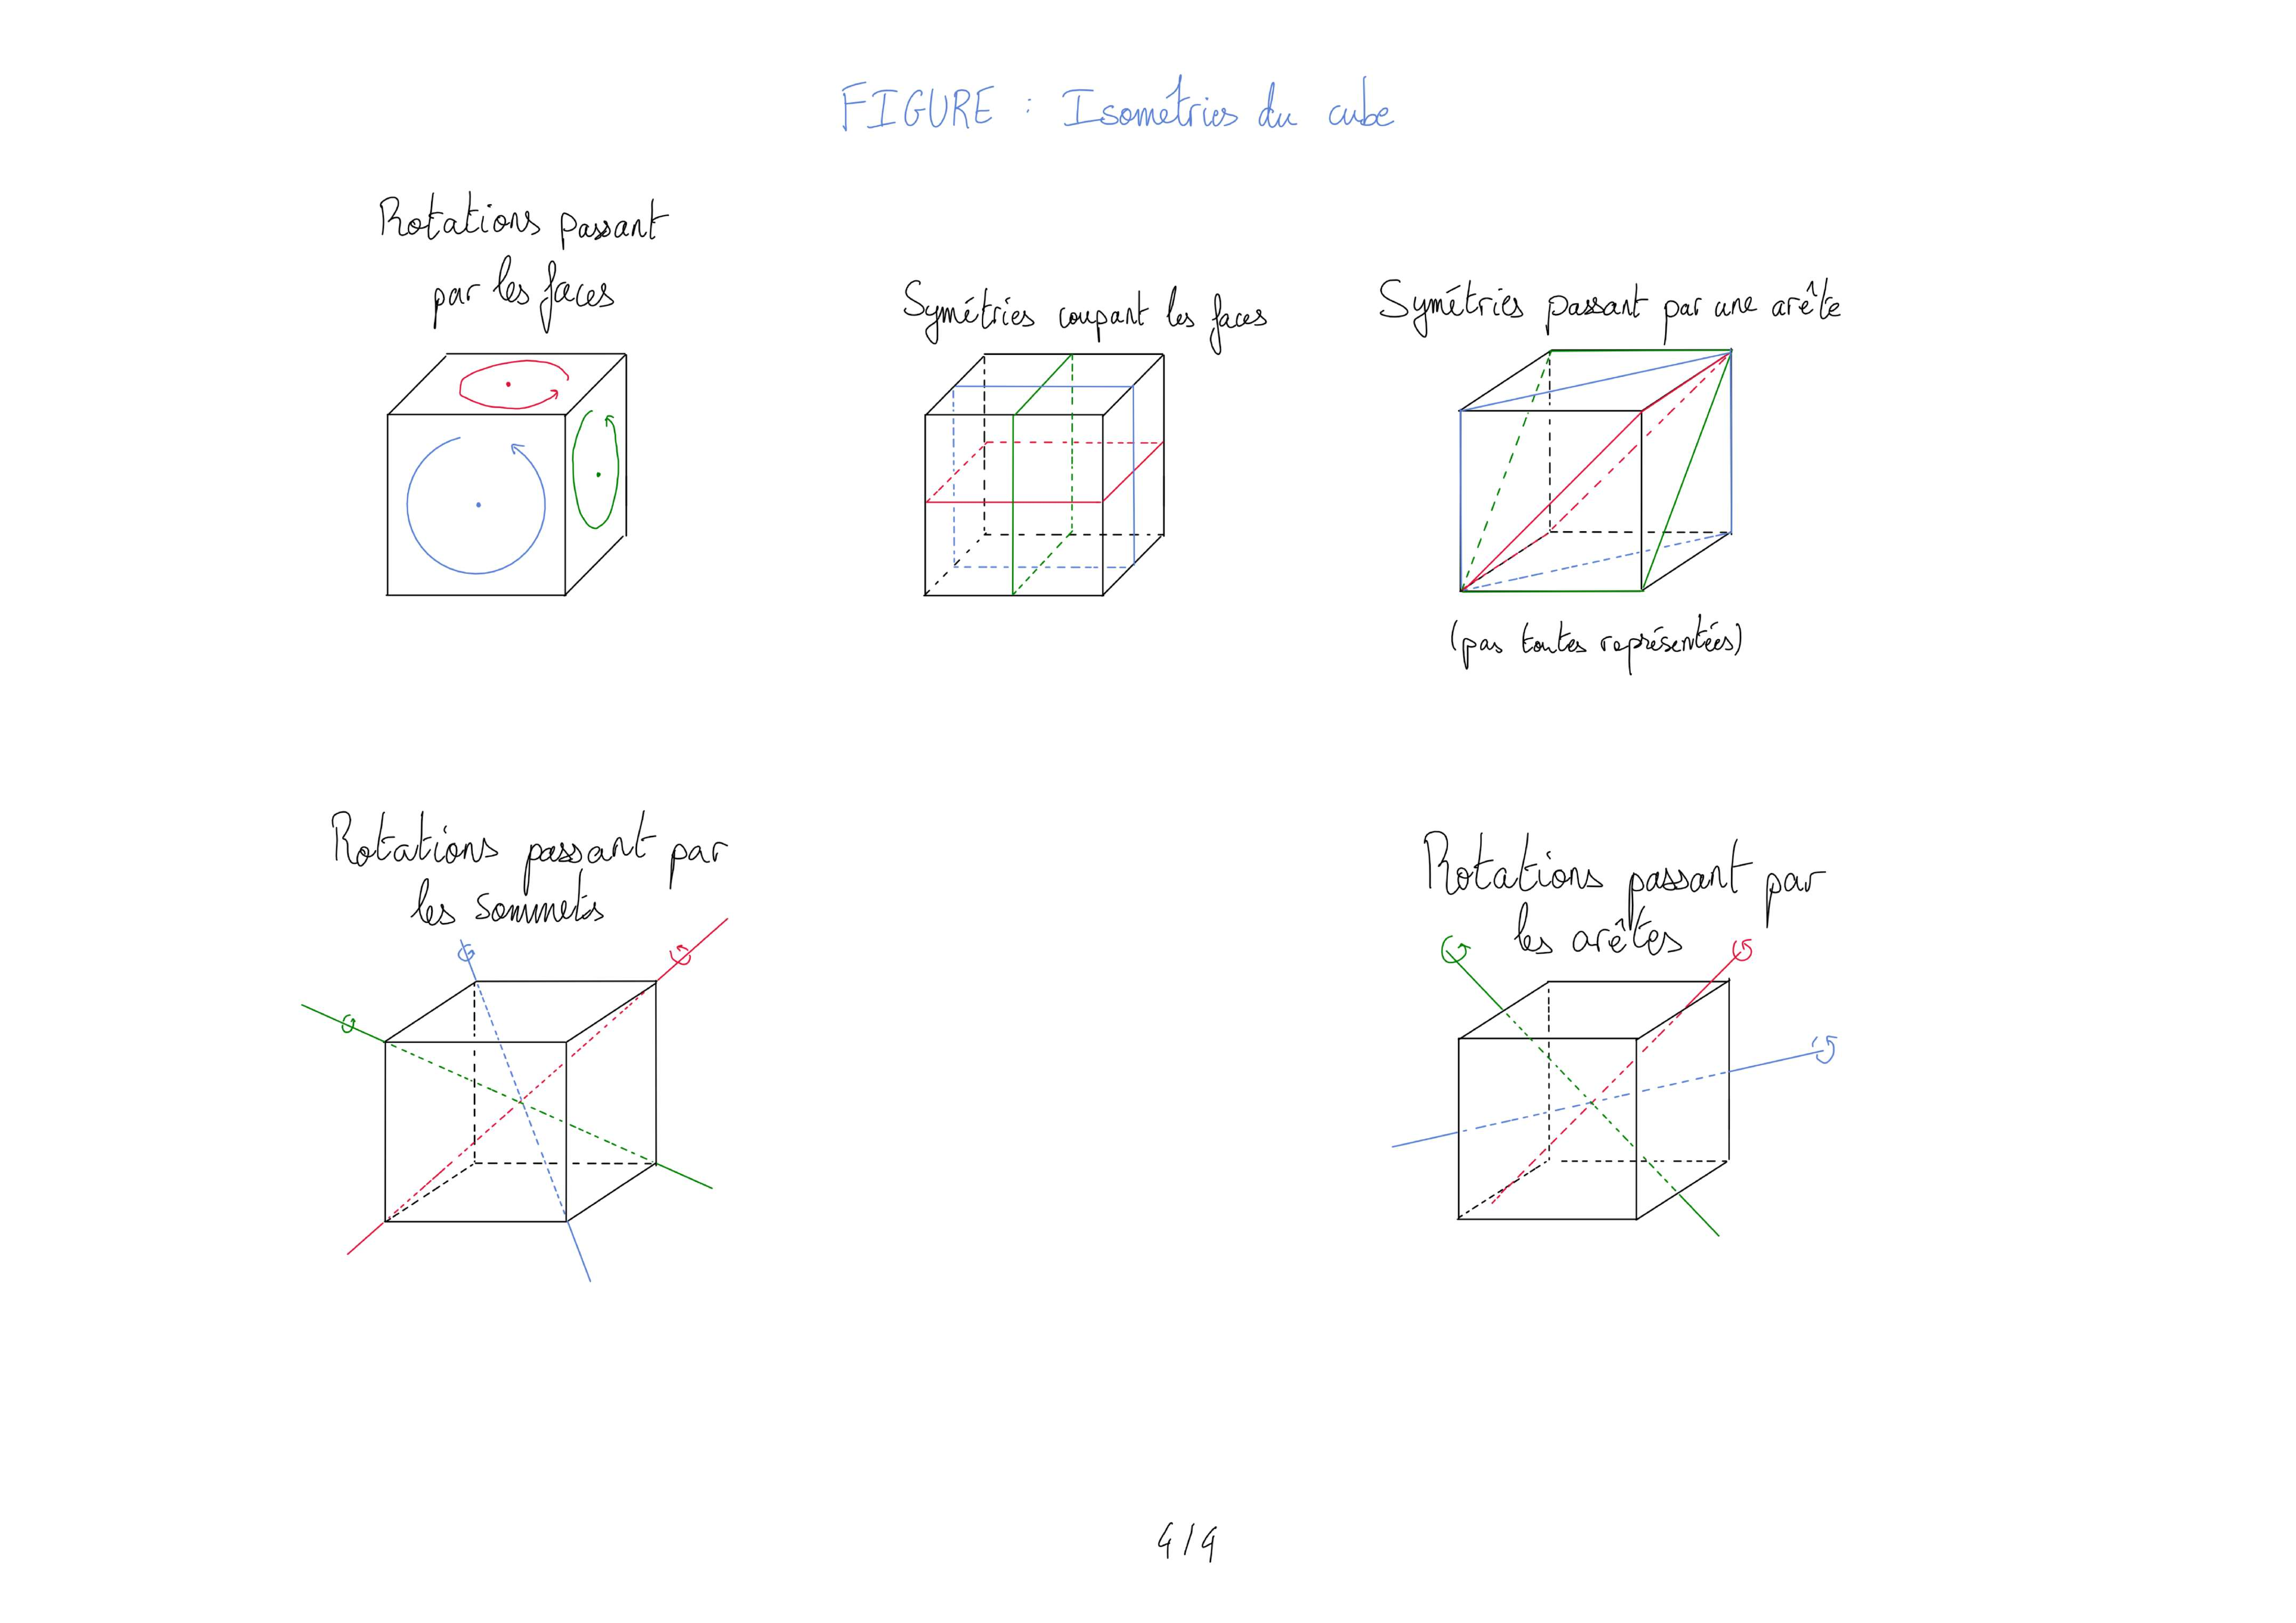
\includegraphics[trim={0 0 0 0},clip,width=1\linewidth]{img/101.pdf}
\end{figure}

\end{document}
